\documentclass{article}
\usepackage{ctex}
\usepackage{geometry}
\geometry{top = 2cm, left = 1cm, right = 1cm, bottom = 2cm}
\usepackage{amsmath,amssymb,amsthm,amsfonts}
\usepackage{abstract}
\usepackage{siunitx}
\usepackage{graphicx}
\usepackage{booktabs}
\usepackage{appendix}
\usepackage{hyperref}
\usepackage{lscape}
\usepackage{multirow}
\usepackage{tikz}

\renewcommand{\appendixpagename}{附录}


\title{卢瑟福散射}
\author{钱思天 2001112187}
\begin{document}
    \maketitle
    \begin{abstract}
        本实验利用了卢瑟福散射仪器,测量了$^{241}\text{Am}$放射源的$\alpha$粒子在金箔上的不同散射角度的分布。通过对散射粒子的测量得到微分散射截面,并与理论结果比较,验证了卢瑟福散射的结论。
        \newline
        \newline
        {\emph{ 关键词:\ 卢瑟福散射、步进电机、$\alpha$粒子 }\rm}

    \end{abstract}

\section{实验原理}

卢瑟福散射的基本思想:$\alpha$粒子被看做一带电质点,在核库仑场中的运动遵从经典运动方程;原子核的大小和原子相比是很小的,且原子核具有正电荷$Ze$和原子的大部分质量;电子的质量很小,对$\alpha$粒子运动的影响可忽略不计。
\begin{enumerate}
  \item 瞄准距离与散射角的关系

  卢瑟福把$\alpha$粒子和靶原子都当做点电荷,假设两者之间的静电斥力是唯一的相互作用力。这是一个两体碰撞问题,如图\ref{fig:IP},设$\alpha$粒子以速度$v_0$沿AT方向入射,由于受到靶核电荷的库仑场作用,$\alpha$粒子将沿轨道ABC运动,即发生了散射。因原子核的质量比$\alpha$粒子的质量大得多,可近似认为靶核静止不动。按库仑定律,相距为$r$的$\alpha$粒子与原子核之间的库仑斥力的大小为:
  
  \begin{equation}
    F = \frac{2Ze^2}{4\pi\varepsilon_0r^2}
  \end{equation}
  
  式中$Z$为靶核电荷数。$\alpha$粒子的轨道为双曲线的一支,如图一所示,原子核与$\alpha$粒子入射方向之间的垂直距离$b$称为瞄准距离(碰撞参数),是入射方向与散射方向之间的夹角。
  
  由牛顿第二定律,可以导出散射角和瞄准距离之间的关系为:
  
  \begin{equation}
    \cos\theta = \frac{2b}{D}
  \end{equation}
  
  其中$D = \frac{1}{4\pi\varepsilon_0}\frac{2Ze^2}{mv^2/2}$。$m$为$\alpha$粒子质量。
  \begin{figure}[htbp]
    \centering



\tikzset{every picture/.style={line width=0.75pt}} %set default line width to 0.75pt        

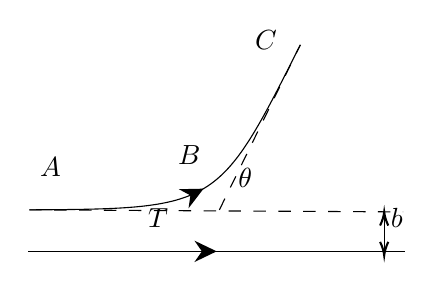
\begin{tikzpicture}[x=0.75pt,y=0.75pt,yscale=-1,xscale=1]
%uncomment if require: \path (0,300); %set diagram left start at 0, and has height of 300

%Straight Lines [id:da09627266306331572] 
\draw    (99.5,150) -- (281.1,150) ;
\draw [shift={(190.3,150)}, rotate = 180] [fill={rgb, 255:red, 0; green, 0; blue, 0 }  ][line width=0.08]  [draw opacity=0] (10.72,-5.15) -- (0,0) -- (10.72,5.15) -- (7.12,0) -- cycle    ;
%Straight Lines [id:da9463203637707641] 
\draw  [dash pattern={on 4.5pt off 4.5pt}]  (100,130) -- (280.1,131) ;
%Curve Lines [id:da251852450217003] 
\draw    (100,130) .. controls (190.6,129.5) and (191.1,129) .. (230.6,50.5) ;
\draw [shift={(183.97,119.8)}, rotate = 513.0899999999999] [fill={rgb, 255:red, 0; green, 0; blue, 0 }  ][line width=0.08]  [draw opacity=0] (10.72,-5.15) -- (0,0) -- (10.72,5.15) -- (7.12,0) -- cycle    ;
%Straight Lines [id:da6578857625233695] 
\draw  [dash pattern={on 4.5pt off 4.5pt}]  (191.6,130) -- (230.6,50.5) ;
%Straight Lines [id:da5053212812635249] 
\draw    (271,133) -- (271,150) ;
\draw [shift={(271,152)}, rotate = 270] [color={rgb, 255:red, 0; green, 0; blue, 0 }  ][line width=0.75]    (6.56,-1.97) .. controls (4.17,-0.84) and (1.99,-0.18) .. (0,0) .. controls (1.99,0.18) and (4.17,0.84) .. (6.56,1.97)   ;
\draw [shift={(271,131)}, rotate = 90] [color={rgb, 255:red, 0; green, 0; blue, 0 }  ][line width=0.75]    (6.56,-1.97) .. controls (4.17,-0.84) and (1.99,-0.18) .. (0,0) .. controls (1.99,0.18) and (4.17,0.84) .. (6.56,1.97)   ;

% Text Node
\draw (199.5,108.5) node [anchor=north west][inner sep=0.75pt]    {$\theta $};
% Text Node
\draw (273,128) node [anchor=north west][inner sep=0.75pt]    {$b$};
% Text Node
\draw (104,103.5) node [anchor=north west][inner sep=0.75pt]    {$A$};
% Text Node
\draw (156,128) node [anchor=north west][inner sep=0.75pt]    {$T$};
% Text Node
\draw (170.5,98) node [anchor=north west][inner sep=0.75pt]    {$B$};
% Text Node
\draw (207.5,42.5) node [anchor=north west][inner sep=0.75pt]    {$C$};


\end{tikzpicture}
\caption{散射角与碰撞参数的关系\label{fig:IP}}

  \end{figure}
  
  \item   卢瑟福的微分散射截面

  有散射角与瞄准距离的关系式(2)可见,瞄准距离$b$增大,散射角就小;反之,$b$小,就大。只要瞄准距离$b$足够小,就可以足够大,这就解释了大角度散射的可能性。但要从实验上验证公式(2),显然是不可能的,因为我们无法测量瞄准距离$b$,然而我们可以求出$\alpha$粒子按瞄准距离的分布,根据这种分布和式(2),就可以推出散射$\alpha$粒子的角分布,而这个角分布是可以直接测量到的。
  
  设有截面为$S$的$\alpha$粒子束射到厚度为$t$的靶上.其中某一$\alpha$粒子的通过靶时相对于靶中某一原子核的瞄准距离在之间的概率,应等于圆周半径分别为$b\sim b+db$圆环面积与入射粒子截面$S$之比.若靶的原子密度为$n$,则$\alpha$粒子束所经过的这块体积内共有$nSt$个原子核,因此,该$\alpha$粒子相对于靶中任一原子核的瞄准距离在$b$与$db$之间的概率为:
  \begin{equation}
    d\omega = \frac{2\pi bdb}{S}nSt = 2\pi n b db
  \end{equation}
  
  这也就是该$\alpha$粒子被散射到$\theta$和$d\theta$之间的概率.
  
  对(2)式求微分,得到
  \begin{equation}
    b|db| = \frac{1}{2}(\frac{D}{2})^2\frac{\cos(\theta/2)}{\sin^3(\theta/2)}d\theta
  \end{equation}
  于是
  \begin{equation}
    d\omega = \pi nt(\frac{D}{2})^2\frac{\cos(\theta/2)}{\sin^3(\theta/2)}d\theta
  \end{equation}
  另外,由角度为$\theta$和$d\theta$的两个圆锥面所围成的立体角可表示为
  \begin{equation}
    d\Omega = \frac{dA}{r^2} = 2\pi\sin\theta d\theta
  \end{equation}
  因此,$\alpha$粒子被散射到该范围内的单位立体角的概率为
  \begin{equation}
    \frac{d\omega}{d\Omega} = nt(\frac{D}{4})^2\frac{1}{\sin^4(\theta/2)}
  \end{equation}
  上式除以单位面积内的靶原子数$nt$可得到微分散射截面
  \begin{equation}
    \frac{d\sigma}{d\Omega} = (\frac{D}{4})^2\frac{1}{\sin^4(\theta/2)}=(\frac{1}{4\pi\varepsilon_0})^2(\frac{Ze^2}{mv_0^2})^2\frac{1}{\sin^4(\theta/2)}
  \end{equation}
  
  实验过程中,设探测器的灵敏面积对靶所张的立体角为$\Delta\Omega$,由卢瑟福散射公式可知在某段时间间隔内所观察到的$\alpha$粒子数$N$应为
  \begin{equation}
    N = (\frac{1}{4\pi\varepsilon_0})^2(\frac{Ze^2}{mv_0^2})^2\frac{\Delta\Omega}{\sin^4(\theta/2)}ntT
  \end{equation}
  式中$T$为该时间内射到靶上的$\alpha$粒子总数.由于式中$N$、$\Delta\Omega$、$\theta$等都是可观测的,所以式(9)可以和实验进行比较。由该式可见,在$\theta$方向上内所观测到$\alpha$粒子数$N$与散射靶的核电荷数$Z$、$\alpha$粒子动能$\frac{1}{2}mv_0^2$及散射角$\theta$等因素都有关,其中$N$正比于$\frac{1}{\sin^4(\theta/2)}$的关系是卢瑟福理论的最有力的验证。
  
\end{enumerate}
\section{实验介绍}
\subsection{实验装置}
卢瑟福散射实验装置主要包括散射真空室部分、电子学系统部分和步进电机的控制系统部分。下面分别介绍。

\begin{enumerate}

\item 散射真空室
\item 
散射真空室主要包括有$\alpha$放射源、散射样品台,Au-Si面垒半导体$\alpha$射线探测器、步进电机及传动装置等。放射源为$^{241}\text{Am}$,主要出射$\alpha$粒子的能量为$5.486\si{MeV}$。真空室是和机械泵相连,开启机械泵后使靶室处于真空状态。

\item
  电子学系统

电子学系统包括灵敏电荷前置放大器(在靶室内)、主放大器、双路定标计数器、探测器偏压电源、低压电源等。此外,在系统的调试过程中,还要用到脉冲信号发生器、示波器和多道分析器等.

\item
  步进电机及其控制系统

在实验过程中,需在真空条件下测量不同散射角的出射$\alpha$粒子计数率,这样就需要不断地转换散射角,在本实验装置中利用步进电机是散射靶转动到来控制散射角,可使实验进行过程变得极为方便,即只需在真空室外控制步进电机转动相应的角度,步进电机精度可靠。可以准确定位。

\end{enumerate}


\subsection{实验操作}

本实验所用放射源为$^{241}\text{Am}$,活度为$0.2\si{mCi}$。

\begin{enumerate}
\item
  检查连线是否正常,用示波器监测是否有异常信号。
\item
  确定散射角$\theta=0^\circ$的物理位置。

打开靶室,转动步进电机;确定push键“按下”与“弹出”对应的转动角的正负关系:找出+方向,给出大约$0^{\circ}$的位置。加上本底盘后,盖上靶室盖,加偏压$80\si{V}$,并抽真空。在为$\pm 10^\circ$范围内,每隔$1^\circ$测一次数,根据峰值确定真正的$\theta=0^\circ$的物理位置。(计数时间为$30\si{s}$)

\item
  测量不同散射角度处本底散射$\alpha$粒子数。

真空下,分别测+方向$\theta=20^\circ,25^\circ,30^\circ,35^\circ,40^\circ,45^\circ,50^\circ$时的计数。(计数时间为$600\si{s}$)

\item
  测量有金箔靶时不同角度对应的散射$\alpha$粒子数。

退掉偏压,停止抽真空,向靶室放气(注意:一定要缓慢放气);然后打开靶室,加上金箔靶,盖上靶室上盖,并抽真空,同时加偏压到$80\si{V}$。重复步骤2,重新确定$\theta=0^\circ$的物理位置后(避免螺旋距差),分别测量+方向$\theta=20^\circ,25^\circ,30^\circ,35^\circ,40^\circ,45^\circ,50^\circ$时的计数。(计数时间为$600\si{s}$)

\item
  用加上金箔靶时的计数减去本底计数,即得从金箔上散射的$\alpha$粒子计数。以散射角为横坐标,散射计数为纵坐标作图,以函数形式N对实验数据进行拟合,并在同一坐标上画出拟合曲线。
\item
  退掉偏压,停止抽真空,向靶室放气(注意:一定要缓慢放气,以免冲破金箔),打开靶室,取出金箔,关掉电源。
\end{enumerate}

\section{实验记录与数据处理}

\subsection{物理原点的确定}

偏压$80\si{V}$,测量时间$30\si{s}$。取逆时针旋转为正,顺时针旋转为负。原点测定的数据如表\ref{tab:1}。
\begin{table}[htbp]
  \centering
  \caption{本底测量的原点标定\label{tab:1}}
  \begin{tabular}{rrrr}
\toprule
 Degree &  Count &  Degree &  Count \\
\midrule
    -10 &   1400 &       1.0 &  29148.0 \\
     -9 &   3169 &       2.0 &  28206.0 \\
     -8 &   5460 &       3.0 &  26948.0 \\
     -7 &   9434 &       4.0 &  25646.0 \\
     -6 &  12398 &       5.0 &  23441.0 \\
     -5 &  17243 &       6.0 &  21836.0 \\
     -4 &  20354 &       7.0 &  18736.0 \\
     -3 &  24540 &       8.0 &  17042.0 \\
     -2 &  27074 &       9.0 &  13331.0 \\
     -1 &  28412 &      10.0 &  10628.0 \\
      0 &  29291 &       -- &      -- \\
\bottomrule
\end{tabular}

\end{table}
通过数据可以看出,当$0^\circ$时计数达到最大,说明$0^\circ$对应着物理零点。

\subsection{本底计数的测量}

测量时间$600\si{s}$。数据记录如表\ref{tab:2}。
\begin{table}[htbp]
  \centering
  \caption{本底测量\label{tab:2}}
  \begin{tabular}{rrr}
\toprule
 DegreeOrigin &  DegreeReal &  Count \\
\midrule
           20 &          20 &     81 \\
           25 &          25 &     16 \\
           30 &          30 &      5 \\
           35 &          35 &      1 \\
           40 &          40 &      0 \\
           45 &          45 &   \color{red}{1999} \\
           50 &          50 &   \color{red}{4914} \\
\bottomrule
\end{tabular}

\end{table}

在大角度时,由于存在噪声,计数出现异常(标红)。

\subsection{加入金箔靶后,物理原点的确定}

测量时间$30\si{s}$。
原点测定的数据如表\ref{tab:3}。
\begin{table}[htbp]
  \centering
  \caption{金箔散射测量的原点标定\label{tab:3}}
  \begin{tabular}{rrrr}
\toprule
 HV[MV] &  I[nA] &  t[s] &    N \\
\midrule
   1.26 &   2.85 & 75.48 &   89 \\
   1.30 &   2.85 & 77.82 &  956 \\
   1.34 &   2.90 & 72.42 & 1138 \\
   1.38 &   2.95 & 69.70 & 1078 \\
   1.42 &   2.90 & 72.00 &  750 \\
   1.46 &   2.90 & 71.66 &  282 \\
   1.50 &   2.90 & 71.24 &  116 \\
\bottomrule
\end{tabular}

\end{table}
通过数据可以看出,当$2^\circ$时计数达到最大,说明$2^\circ$对应着物理零点,这是由于螺旋距差的影响。

\subsection{金箔靶散射计数的测量}

测量时间$600\si{s}$。数据记录如表\ref{tab:4}。
\begin{table}[htbp]
  \centering
  \caption{金箔散射信号测量\label{tab:4}}
  \begin{tabular}{rrrr}
\toprule
  HV[MV] &    N &      Deepth[\AA] &  H Percent \\
\midrule
1.26 &   89 & -317.32 &   0.79\% \\
1.30 &  956 &  226.98 &   8.43\%\\
1.34 & 1138 &  806.89 &  10.03\% \\
1.38 & 1078 & 1376.05 &   9.51\% \\
1.42 &  750 & 1896.76 &   6.61\% \\
1.46 &  282 & 2362.91 &   2.49\% \\
1.50 &  116 & 2861.96 &   1.02\% \\
\bottomrule
\end{tabular}

\end{table}

在大角度时,由于存在噪声,计数出现异常(标红)。



\subsection{验证卢瑟福散射公式}

根据2、4步的测量结果,计算散射$\alpha$粒子的计数(舍去标红的噪声较大的数据点)对其进行线性拟合,得到的拟合曲线如图\ref{fig:Fit}。
\begin{figure}[htbp]
  \centering
  \includegraphics[width=0.7\textwidth]{../plots/Fit.pdf}
  \caption{拟合计数图\label{fig:Fit}}
\end{figure}

可以看出,虽然计数的误差很大,但是整体上看,散射$\alpha$计数$N$与$\frac{\mathbf{1}}{\mathbf{\sin}^{\mathbf{4}}\frac{\mathbf{\theta}}{\mathbf{2}}}$基本呈线性关系,定性上验证了公式(9)。
\section{致谢}
    感谢赵捷老师的指导。 
    \clearpage
    \appendix
    \appendixpage
    \section{思考题:(一)}


1.
散射$\alpha$粒子计数$N$与散射角\(\theta\)。通过测量不同的散射角\(\theta\)下散射$\alpha$粒子计数$N$以确定二者的关系。

2.实验需要验证的关系是散射$\alpha$粒子计数$N$与\(\frac{\mathbf{1}}{\mathbf{\sin}^{\mathbf{4}}\frac{\mathbf{\theta}}{\mathbf{2}}}\)线性关系,公式中的\(\theta\)是以物理零点作为基准确定的,所以需要进行零点校准。首先打开本底盖,大致找出\(\theta = 0{^\circ}\)的位置,在\(\pm 10{^\circ}\)的范围内,每隔\(1{^\circ}\)测量一个散射计数,计数峰值对应的散射角度就是物理原点。同时,尽量让一次测量(本底或者信号)下步进马达沿同一个方向运动,这样可以避免螺距差。打开本底盖,在显示为+时按下start,观察电机转动方向,确定逆时针为\(+ \theta\)方向。

3.
散射$\alpha$粒子计数N\(与\frac{\mathbf{1}}{\mathbf{\sin}^{\mathbf{4}}\frac{\mathbf{\theta}}{\mathbf{2}}}\)基本呈线性关系,\(\theta\)较小时,计数太大。散射角度从\(20{^\circ}\)变到\(25{^\circ}\),散射计数迅速下降。

4.可以用计数的平方根作为Poisson分布的误差。

5.实验结果跟理论线符合的很差,主要是因为存在极大的噪声,几乎淹没了信号。
\section{思考题:(二)}

从式(9)可以看出散射$\alpha$粒子计数$N$与\(\frac{1}{\sin^{4}\frac{\theta}{2}}\)的线性相关系数既与靶原子序数的平方成正比,又与单位面积上的靶原子的原子序数成正比。因此通过用$\alpha$粒子轰击未知靶,然后测量不同的散射角\(\theta\)下散射$\alpha$粒子计数$N$,可以得到$N$与\(\frac{1}{\sin^{4}\frac{\theta}{2}}\)的线性拟合关系。再通过与标准核(如金箔的散射结果)比较,就可以获得未知靶核的信息。
\end{document}